\documentclass[border=6pt]{standalone}
% Shared TikZ styles for the network diagrams.
\usepackage{tikz}
\usetikzlibrary{arrows.meta,positioning}
\definecolor{nodeblue}{HTML}{2A78D6}
\definecolor{endfill}{HTML}{E3EEFB}
\definecolor{shortcut}{HTML}{D64545}
\tikzset{
  v/.style={circle, draw=nodeblue, line width=1pt, minimum size=9mm, inner sep=0pt, font=\small},
  od/.style={v, fill=endfill},
  e/.style={-{Latex[length=2.6mm]}, line width=0.8pt},
  free/.style={e, shortcut},
  c/.style={font=\footnotesize, fill=white, inner sep=1.5pt},
}

\begin{document}
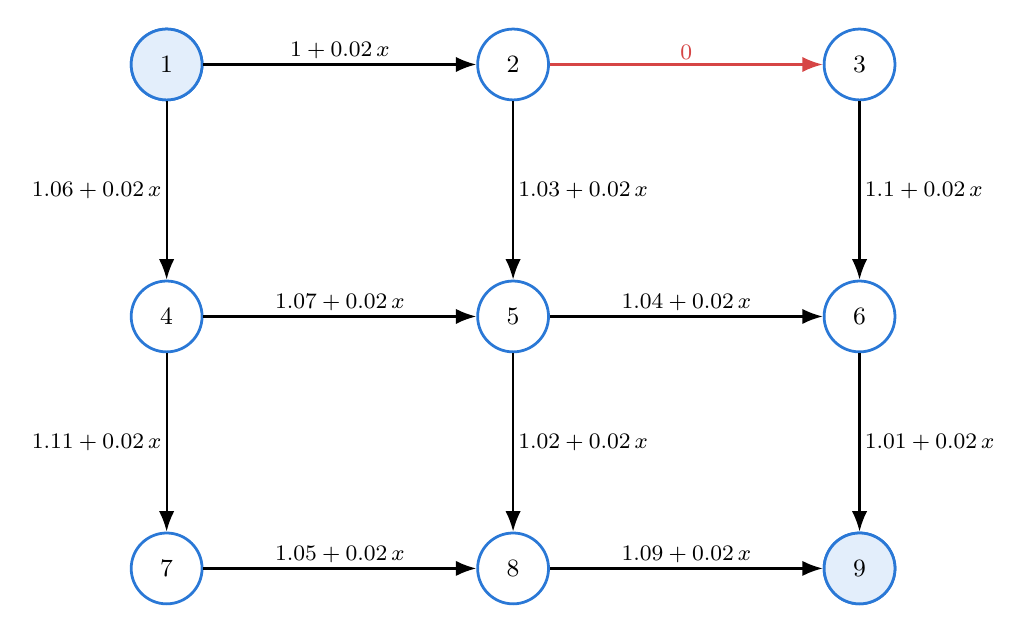
\begin{tikzpicture}[x=4.4cm, y=-3.2cm]
  \foreach \n [count=\i from 0] in {1,...,9} {
    \pgfmathtruncatemacro\col{mod(\i,3)}
    \pgfmathtruncatemacro\row{div(\i,3)}
    \node[v] (\n) at (\col,\row) {\n};
  }
  \node[od] at (1) {1};
  \node[od] at (9) {9};
  % horizontal edges
  \draw[e]    (1) -- node[c, above] {$1 + 0.02\,x$}    (2);
  \draw[free] (2) -- node[c, above] {$0$}              (3);
  \draw[e]    (4) -- node[c, above] {$1.07 + 0.02\,x$} (5);
  \draw[e]    (5) -- node[c, above] {$1.04 + 0.02\,x$} (6);
  \draw[e]    (7) -- node[c, above] {$1.05 + 0.02\,x$} (8);
  \draw[e]    (8) -- node[c, above] {$1.09 + 0.02\,x$} (9);
  % vertical edges
  \draw[e] (1) -- node[c, left]  {$1.06 + 0.02\,x$} (4);
  \draw[e] (4) -- node[c, left]  {$1.11 + 0.02\,x$} (7);
  \draw[e] (2) -- node[c, right] {$1.03 + 0.02\,x$} (5);
  \draw[e] (5) -- node[c, right] {$1.02 + 0.02\,x$} (8);
  \draw[e] (3) -- node[c, right] {$1.1 + 0.02\,x$}  (6);
  \draw[e] (6) -- node[c, right] {$1.01 + 0.02\,x$} (9);
\end{tikzpicture}
\end{document}
